\documentclass[conference]{IEEEtran}
% \IEEEoverridecommandlockouts
% The preceding line is only needed to identify funding in the first footnote. If that is unneeded, please comment it out.
%Template version as of 6/27/2024

\usepackage{amsmath,amssymb,amsfonts}
\usepackage{algorithmic}
\usepackage{graphicx}
\usepackage{textcomp}
\usepackage{xcolor}
\usepackage[style=ieee,url=false,doi=false,isbn=false,eprint=true]{biblatex}
\addbibresource{../references.bib}
%\renewcommand{\arraystretch}{1.2} % vertical padding in table

\begin{document}
\title{Unsupervised Model Transfer Between Temperature-Modulated MOX Gas Sensors}

\makeatletter
\newcommand{\linebreakand}{%
  \end{@IEEEauthorhalign}
  \hfill\mbox{}\par
  \mbox{}\hfill\begin{@IEEEauthorhalign}
}
\makeatother

\author{\IEEEauthorblockN{Brady Laska (SMIEEE)}
\IEEEauthorblockA{\textit{Systems and Computer Engineering} \\
\textit{SAM\textsuperscript{3} Innovation Hub}\\
\textit{Carleton University}\\
Ottawa, Canada \\
laska@sce.carleton.ca}
\and
\IEEEauthorblockN{Julio J. Valdés (SMIEEE)}
\IEEEauthorblockA{\textit{National Research Council Canada} \\
Ottawa, Canada \\
julio.valdes@nrc-cnrc.gc.ca}
\and
\IEEEauthorblockN{Yuxin Kang}
\IEEEauthorblockA{\textit{National Research Council Canada} \\
Ottawa, Canada \\
}
\and
\linebreakand
\IEEEauthorblockN{Antoine Guirguis}
\IEEEauthorblockA{\textit{Systems and Computer Engineering} \\
\textit{SAM\textsuperscript{3} Innovation Hub}\\
\textit{Carleton University}\\
Ottawa, Canada \\
AntoineGuirguis3@cunet.carleton.ca}
\and
\IEEEauthorblockN{Rafik Goubran (LFIEEE)}
\IEEEauthorblockA{\textit{Systems and Computer Engineering} \\
\textit{SAM\textsuperscript{3} Innovation Hub}\\
\textit{Carleton University}\\
Ottawa, Canada \\
goubran@sce.carleton.ca}
\and
\IEEEauthorblockN{Pengcheng Xi (MIEEE)}
\IEEEauthorblockA{\textit{National Research Council Canada} \\
Ottawa, Canada \\
Pengcheng.Xi@nrc-cnrc.gc.ca}
}

\maketitle

\begin{abstract}
    Variability between nominally identical metal-oxide semiconductor (MOX) gas sensors limits the transfer of odor classification models between devices. This work investigates unsupervised domain adaptation for temperature-modulated MOX sensors using unlabeled exposure data, without requiring measurements under known reference conditions. We collected over 26,000 measurement cycles from eight sensors exposed simultaneously to 37 substances spanning nuts, herbs, and spices, with two sensors assigned to each of four heater profiles. Using linear discriminant analysis, we evaluate classification transfer between paired sensors and compare compensation methods ranging from scalar mean subtraction to full covariance alignment. With log-resistance and log-vapor-pressure features, per-heater-step mean compensation increases mean target balanced accuracy from 47.0\% to 68.4\% across eight transfer directions, while CORAL-style covariance alignment achieves 71.2\%. Including vapor pressure improves performance under every compensation method. Per-step mean compensation retains most of its full-coverage performance when adaptation statistics are estimated from only five substances, and transfer improvements extend to substances excluded from adaptation. These results indicate that per-heater-step offsets account for much of the sensor mismatch under shared exposure conditions, allowing simple adjustments estimated from unlabeled measurements to substantially improve model transfer.
\end{abstract}

\begin{IEEEkeywords}
    e-nose, gas sensor, calibration, classification, machine learning
\end{IEEEkeywords}

\section{Introduction}
Metal-oxide semiconductor (MOX) gas sensors are widely used for embedded smell sensing because of their low cost, small size, and sensitivity to volatile compounds. 
Individual sensors can be used to monitor changes in the concentration or composition of volatile gases \cite{verzeroli2025MoxOutdoor}, \cite{laska2025spoilage}.
Combining multiple sensors into an e-nose array, or cycling a single sensor through multiple operating temperatures \cite{lee1999TemperatureModulation}, produces a response signature that can be used to classify odors \cite{hussain2023DLGasClassify}. However, variability between nominally identical sensors can reduce classification accuracy when a model trained on one device is applied to another. Manufacturing variation can produce differences in baseline resistance and sensitivity, while sensor aging and exposure memory effects can change an individual sensor’s response over time \cite{panzardi2025bme688,dennler2022drift}.

Existing approaches to managing MOX sensor variability include calibration transfer and global calibration models. Calibration transfer methods use measurements acquired under known reference conditions to estimate a correction between source and target sensor responses \cite{fernandez2016transfer}, while global calibration models are trained using measurements from multiple sensors \cite{miquelibarz2022global,sumanto2026calibration}.

In this work, we frame sensor variability as a distribution shift between training and deployment datasets and investigate unsupervised domain adaptation for classification model transfer. We estimate adjustments from unlabeled source and target exposure data, without requiring measurements under known reference conditions. We compare methods using increasingly detailed response statistics, from a single mean offset through to full covariance alignment. We also investigate how transfer performance depends on the amount of data used to estimate the adaptation statistics.

To evaluate these methods, we collected approximately 17 hours of simultaneous measurements from eight temperature-modulated MOX sensors exposed to 37 substances spanning nuts, herbs, and spices. Two sensors were assigned to each of four heater profiles, supporting transfer experiments between paired sensors under shared exposure conditions. The dataset contains over 26,000 measurement cycles and allows us to assess adaptation across diverse substance responses.

%\section{Introduction}
%Metal-oxide semiconductor (MOX) gas sensors are popular for embedded smell sensing applications due to their low-cost, compact form, and high sensitivity to volatile compounds \cite{nikolic2020GasSensorReview}. They can be used individually, to monitor changes in the concentration or composition of volatile gasses \cite{verzeroli2025MoxOutdoor}, \cite{laska2025spoilage}, or combined into an array as an e-nose that can measure smell signatures of specific odours \cite{hussain2023DLGasClassify}, \cite{feng2026smellnet}. Since the gas-oxide reactions in a MOX sensor are temperature dependent \cite{lee1999TemperatureModulation}, a single sensor can be temperature-cycled through muiltiple operating points to create a virtual array \cite{parsiegel2025VirtualArray}.
%
%Despite these advantages, MOX sensors have inherent limitations that complicate their use in reliable, long-term smell sensing. Their lack of selectivity, temperature dependent response, and cross-sensitivity to water vapor make them susceptible to variations in environmental conditions, and their slow response time reduces their utility in dynamic environments.
%Sensor variability is another concern, especially when sensors are combined with machine learning models for odor detection or classification. Bulk and surface material defects and manufacturing variation can cause nominally identical sensors to differ significantly in baseline response and sensitivity \cite{panzardi2025bme688}. Sensor aging and exposure memory effects can also alter an individual sensor’s baseline and sensitivity over time \cite{dennler2022drift}. Both sensor-to-sensor variability and temporal drift can shift the distribution of sensor responses relative to the decision boundaries learned during training, reducing classification performance when a model is applied to a different sensor or deployed over time.
%
%Collected large dataset to Explore classification model transfer of temperature modulated MOX sensors using multiple sensors under shared exposure conditions.
%Methods for dealing with sensor variation include Measurements under controlled conditions \cite{fernandez2016transfer}, or using a collection of sensors to build global calibration models \cite{miquelibarz2022global} \cite{sumanto2026calibration}
%In this work, machine learning, domain adaptation.
%We focus on unlabelled data.

\section{Methods}
\subsection{Data collection}
We collected data using an eight-sensor BME-690 evaluation board from Bosch-Sensortec GmbH \cite{boschBME690}. Each BME-690 integrates a MOX gas sensor with a programmable hotplate to control the temperature of the sensing layer, along with sensing elements for temperature and relative humidity on a separate die \cite{panzardi2025bme688}. The firmware supports temperature-cycled operation through ``heating profiles'', where the integrated heater is cycled through a sequence of setpoint temperatures, with measurements captured at specified time offsets. Since the sampling intervals are non-uniform within the cycle, the resistance, temperature, and humidity measurements from each sample point are grouped into a vector reading covering the heater cycle. 

\begin{figure}[tbp]
    \centering
    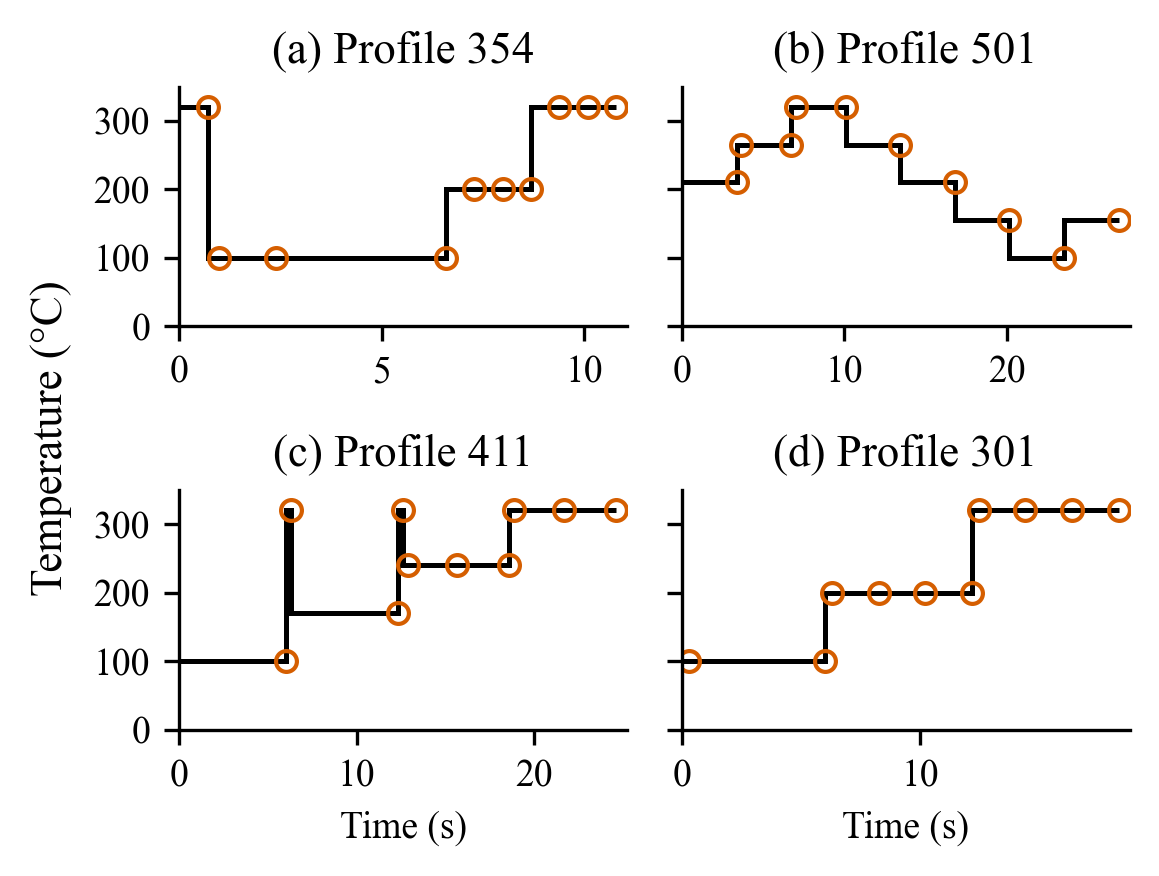
\includegraphics[width=\linewidth]{figures/heater_profiles.png}
    \caption{Heater profiles for BME-690 sensors. The continuous line shows the target temperature of the sensor hotplate; circles indicate sensing times. Figure based on \cite{boschBME690}.}
    \label{fig:heating_profiles}
\end{figure}
We configured the four heating profiles shown in Fig.~\ref{fig:heating_profiles}, the default profiles for the multi-sensor evaluation board, assigning two sensors to each profile as listed in Table \ref{tab:profiles}.
\begin{table}[htbp]
\caption{Sensor and heating profile assignment.}
\label{tab:profiles}
\centering
\begin{tabular}{|c|c|}
    \hline
    \textbf{Sensors} & \textbf{Profile} \\
    \hline
    0, 4 & 354 \\
    1, 5 & 501 \\
    2, 6 & 411 \\
    3, 7 & 301 \\
    \hline
\end{tabular}
\end{table}

All profiles have ten sample points per cycle, but their cycle durations differ, resulting in different numbers of sample vectors per sensor.
We collected simultaneous headspace measurements with all eight sensors exposed to the same substance sample in a closed container. The substance selection and measurement protocol were informed by \cite{feng2026smellnet}. For each substance listed in Table \ref{tab:substance-classes}, we collected measurements during 10 minutes of exposure followed by 10 minutes of recovery in open air. We repeated this sequence at least twice per substance to capture variations in sensor convergence and environmental conditions. The resulting dataset comprises approximately 17 hours of data collected for each of the eight sensors across 37 substance classes.

\begin{table}[htbp]
\caption{Substance classes by category (37 total).}
\label{tab:substance-classes}
\centering
\footnotesize
\begin{tabular}{|p{0.18\columnwidth}|p{\dimexpr0.82\columnwidth-4\tabcolsep-3\arrayrulewidth\relax}|}
\hline
\textbf{Category} & \textbf{Substances} \\
\hline
Nuts (11) &
Almond, cashew, chestnuts, hazelnut, hickory nut,
macadamia, peanuts, pecans, pine nut, pistachios,
walnuts. \\
\hline
Herbs (16) &
Angelica, chives, dried tangerine peel, eupatorium,
gentiana, hops, lavender, lemongrass, lonicera,
mugwort, oregano, rosemary, sage, turnip,
vaccaria seed, vervain. \\
\hline
Spices (10) &
Black pepper, cardamom, cloves, cumin, fennel seed,
ginger, mustard, nutmeg, saffron, star anise. \\
\hline
\end{tabular}
\end{table}

\subsection{Features}
We use MOX-sensor resistance and humidity as classifier features; humidity is included to allow the classifiers to compensate for the cross-sensitivity of the MOX sensor to water vapor.
We compute vapor pressure, $P_v$, from the measured temperature, $T$ (in $^\circ$C), and relative humidity, $RH$ (in percent), as follows \cite{bolton1980computation}:
\begin{equation}
P_v = \frac{RH}{100}\,6.112\exp\left(\frac{17.67T}{T+243.5}\right).
\end{equation}
We log-transform the MOX resistance and vapor pressure to linearize the power-law response of the MOX sensor to volatile gases and water vapor \cite{yamazoe2008theory}. 
The log resistance and log vapor pressure readings from each heating profile step are concatenated into a feature vector covering one complete cycle of the corresponding profile shown in Fig.~\ref{fig:heating_profiles}. Each heating profile has 10 steps, resulting in a 20-element feature vector when both resistance and vapor pressure features are used.

\subsection{Domain Adaptation}
We investigate a range of unsupervised domain adaptation methods that use progressively more information about the source and target distributions.
Domain adaptation targets only the log-resistance features to compensate for variation in the MOX sensors.

\subsubsection{Scalar mean}
Let $\mathbf{u}_s$ denote a source sensor feature vector and $\mathbf{u}_t$ the corresponding vector for the target sensor.
First, we consider a single scalar offset for each sensor:
\begin{equation}
\tilde{\mathbf{u}}_k=\mathbf{u}_k-\mu_k,\ k\in\{s, t\},
\end{equation}
where $\mu_k$ is the average log resistance over all heating profile steps in all samples. This is similar to the approach used in \cite{panzardi2025bme688}, where linear BME-688 responses were normalized as:
\begin{equation} 
    (R(t) - R(0))/R(0)
\end{equation} 
where and $R(0)$ is the sensor resistance in carrier gas at the beginning of a test.

\subsubsection{Vector mean}
Next, we consider per-feature mean subtraction:
\begin{equation}
\tilde{\mathbf{u}}_k=\mathbf{u}_k-\mathbf{m}_k,\ k\in\{s, t\},
\end{equation}
where $\mathbf{m}_k = \mathbb{E}\{\mathbf{u}_k\}$ is the sensor-specific feature mean vector across the compensation dataset.
This compensates for per-sensor baselines at each operating point, but not for variations in sensor sensitivity.

\subsubsection{Vector mean-variance}
Next, we independently standardize the sensor feature vectors to zero mean and unit variance as:
\begin{equation}
\tilde{\mathbf{u}}_k=D_k^{-1}(\mathbf{u}_k-\mathbf{m}_k),\ k\in\{s, t\}
\end{equation}
where $D_k$ is a diagonal matrix of per-feature sample standard deviations. This compensates for differences in feature offsets and scales, corresponding to variations in the sensor baselines and sensitivities at each operating point, but does not consider cross-feature relationships.

\subsubsection{CORAL-type}
Finally, we consider the case where we have the full covariance matrix for the source and target sensors.
CORAL~\cite{sun2016coral} is an unsupervised domain adaptation method that aligns the second-order statistics of source and target distributions without requiring labels on the target dataset. It works by first whitening the source distribution and then re-coloring it with the target covariance. We reverse the original source-to-target mapping and instead transform the target into source coordinates, allowing the source classifier to remain fixed.

The target transform is:
\begin{equation}
\tilde{\mathbf{u}}_t=\mathbf{m}_s+(C_s+\lambda I)^{1/2}(C_t+\lambda I)^{-1/2}(\mathbf{u}_t-\mathbf{m}_t),
\end{equation}
where $C_s$, and $C_t$ are the source and target sample covariance matrices, respectively. We set $\lambda=10^{-3}$ as a fixed regularization parameter, without tuning on target scores.

Table \ref{tab:target-information} summarizes the compensation methods and their required statistics.
\begin{table}[htb]
\centering
\caption{Target information used for adaptation.}
\label{tab:target-information}
\begin{tabular}{|c|l|}
\hline
\textbf{Method} & \textbf{Estimated Statistics} \\
\hline
No target adjustment & None\\
\hline
Scalar mean & Per-sensor mean \\
\hline
Vector mean & Feature means \\
\hline
Vector mean-variance & Feature means and variances \\
\hline
CORAL-style & Feature means and covariance matrix \\
\hline
\end{tabular}
\end{table}


\subsection{Transfer protocol}
Unless otherwise specified, we estimate the distribution statistics from the entire unlabeled source and target datasets. No separate calibration interval is used. We fit a standard scaler to the compensated source features and apply the same transformation to the compensated target features. The uncompensated reference uses the same source-normalized scaling without any target-specific adjustment.

We use linear discriminant analysis (LDA) as a representative classifier, training on one sensor and evaluating on its paired sensor. While more advanced classifiers, such as support vector machines (SVMs), could be considered, we chose LDA as a simple baseline whose performance is less dependent on the choice of hyperparameters. The classifier uses the singular value decomposition solver with empirical source class priors and no hyperparameter tuning. Evaluation covers both transfer directions for each same-profile sensor pair, giving eight directions.
We report accuracy and balanced accuracy, computed as mean recall across the 37 classes. We also report the source training score as a reference to assess the performance drop on the target sensor data.

\subsubsection{Ablation}
We evaluate the contributions of the input features and compensation methods through an ablation study. For features, we consider log resistance alone, log vapor pressure alone, and their combination. For compensation, we consider the methods in Table \ref{tab:target-information}.

\subsubsection{Reduced Data Adaptation}
Next, we evaluate the impact of reducing the amount of data used for adaptation. To simulate the practical scenario where the sensor offsets are computed from an initial limited-exposure calibration period, we vary the number of classes used to estimate the source and target statistics, while using all the classes for classifier training and evaluation. For each number of adaptation classes, we repeat 30 trials with random subsets of classes assigned to the adaptation set. To assess if classs-specific adaptation is necessary, we compare the transfer classification performance for all classes and on the subset of classes that were excluded from adaptation.

% \subsection{Figures and Tables}\label{FAT}
%
% \begin{table}[htbp]
% \caption{Table Type Styles}
% \begin{center}
% \begin{tabular}{|c|c|c|c|}
% \hline
% \textbf{Table}&\multicolumn{3}{|c|}{\textbf{Table Column Head}} \\
% \cline{2-4}
% \textbf{Head} & \textbf{\textit{Table column subhead}}& \textbf{\textit{Subhead}}& \textbf{\textit{Subhead}} \\
% \hline
% copy& More table copy$^{\mathrm{a}}$& &  \\
% \hline
% \multicolumn{4}{l}{$^{\mathrm{a}}$Sample of a Table footnote.}
% \end{tabular}
% \label{tab1}
% \end{center}
% \end{table}

\section{Results}
\subsection{Geometry of Smell Signatures}
Fig.~\ref{fig:lda_heating_profiles} compares LDA projections for four sensors (sensors 0--3) covering the four heating profiles shown in Fig.~\ref{fig:heating_profiles}. For each sensor, we standardize the log-resistance features over all cycles and fit LDA to the 37 substance labels. Each point represents one cycle and color identifies the dataset category (nuts, herbs, or spices). Centroids of select classes are labeled to better visualize the projections. Similarly, the shared plot limits aid comparison between the sensor projections but do not represent common coordinates.
\begin{figure*}[t!bp]
    \centering
    %\includegraphics[width=\textwidth]{../results/single_sensor_lda/sensor_pairs.png}
    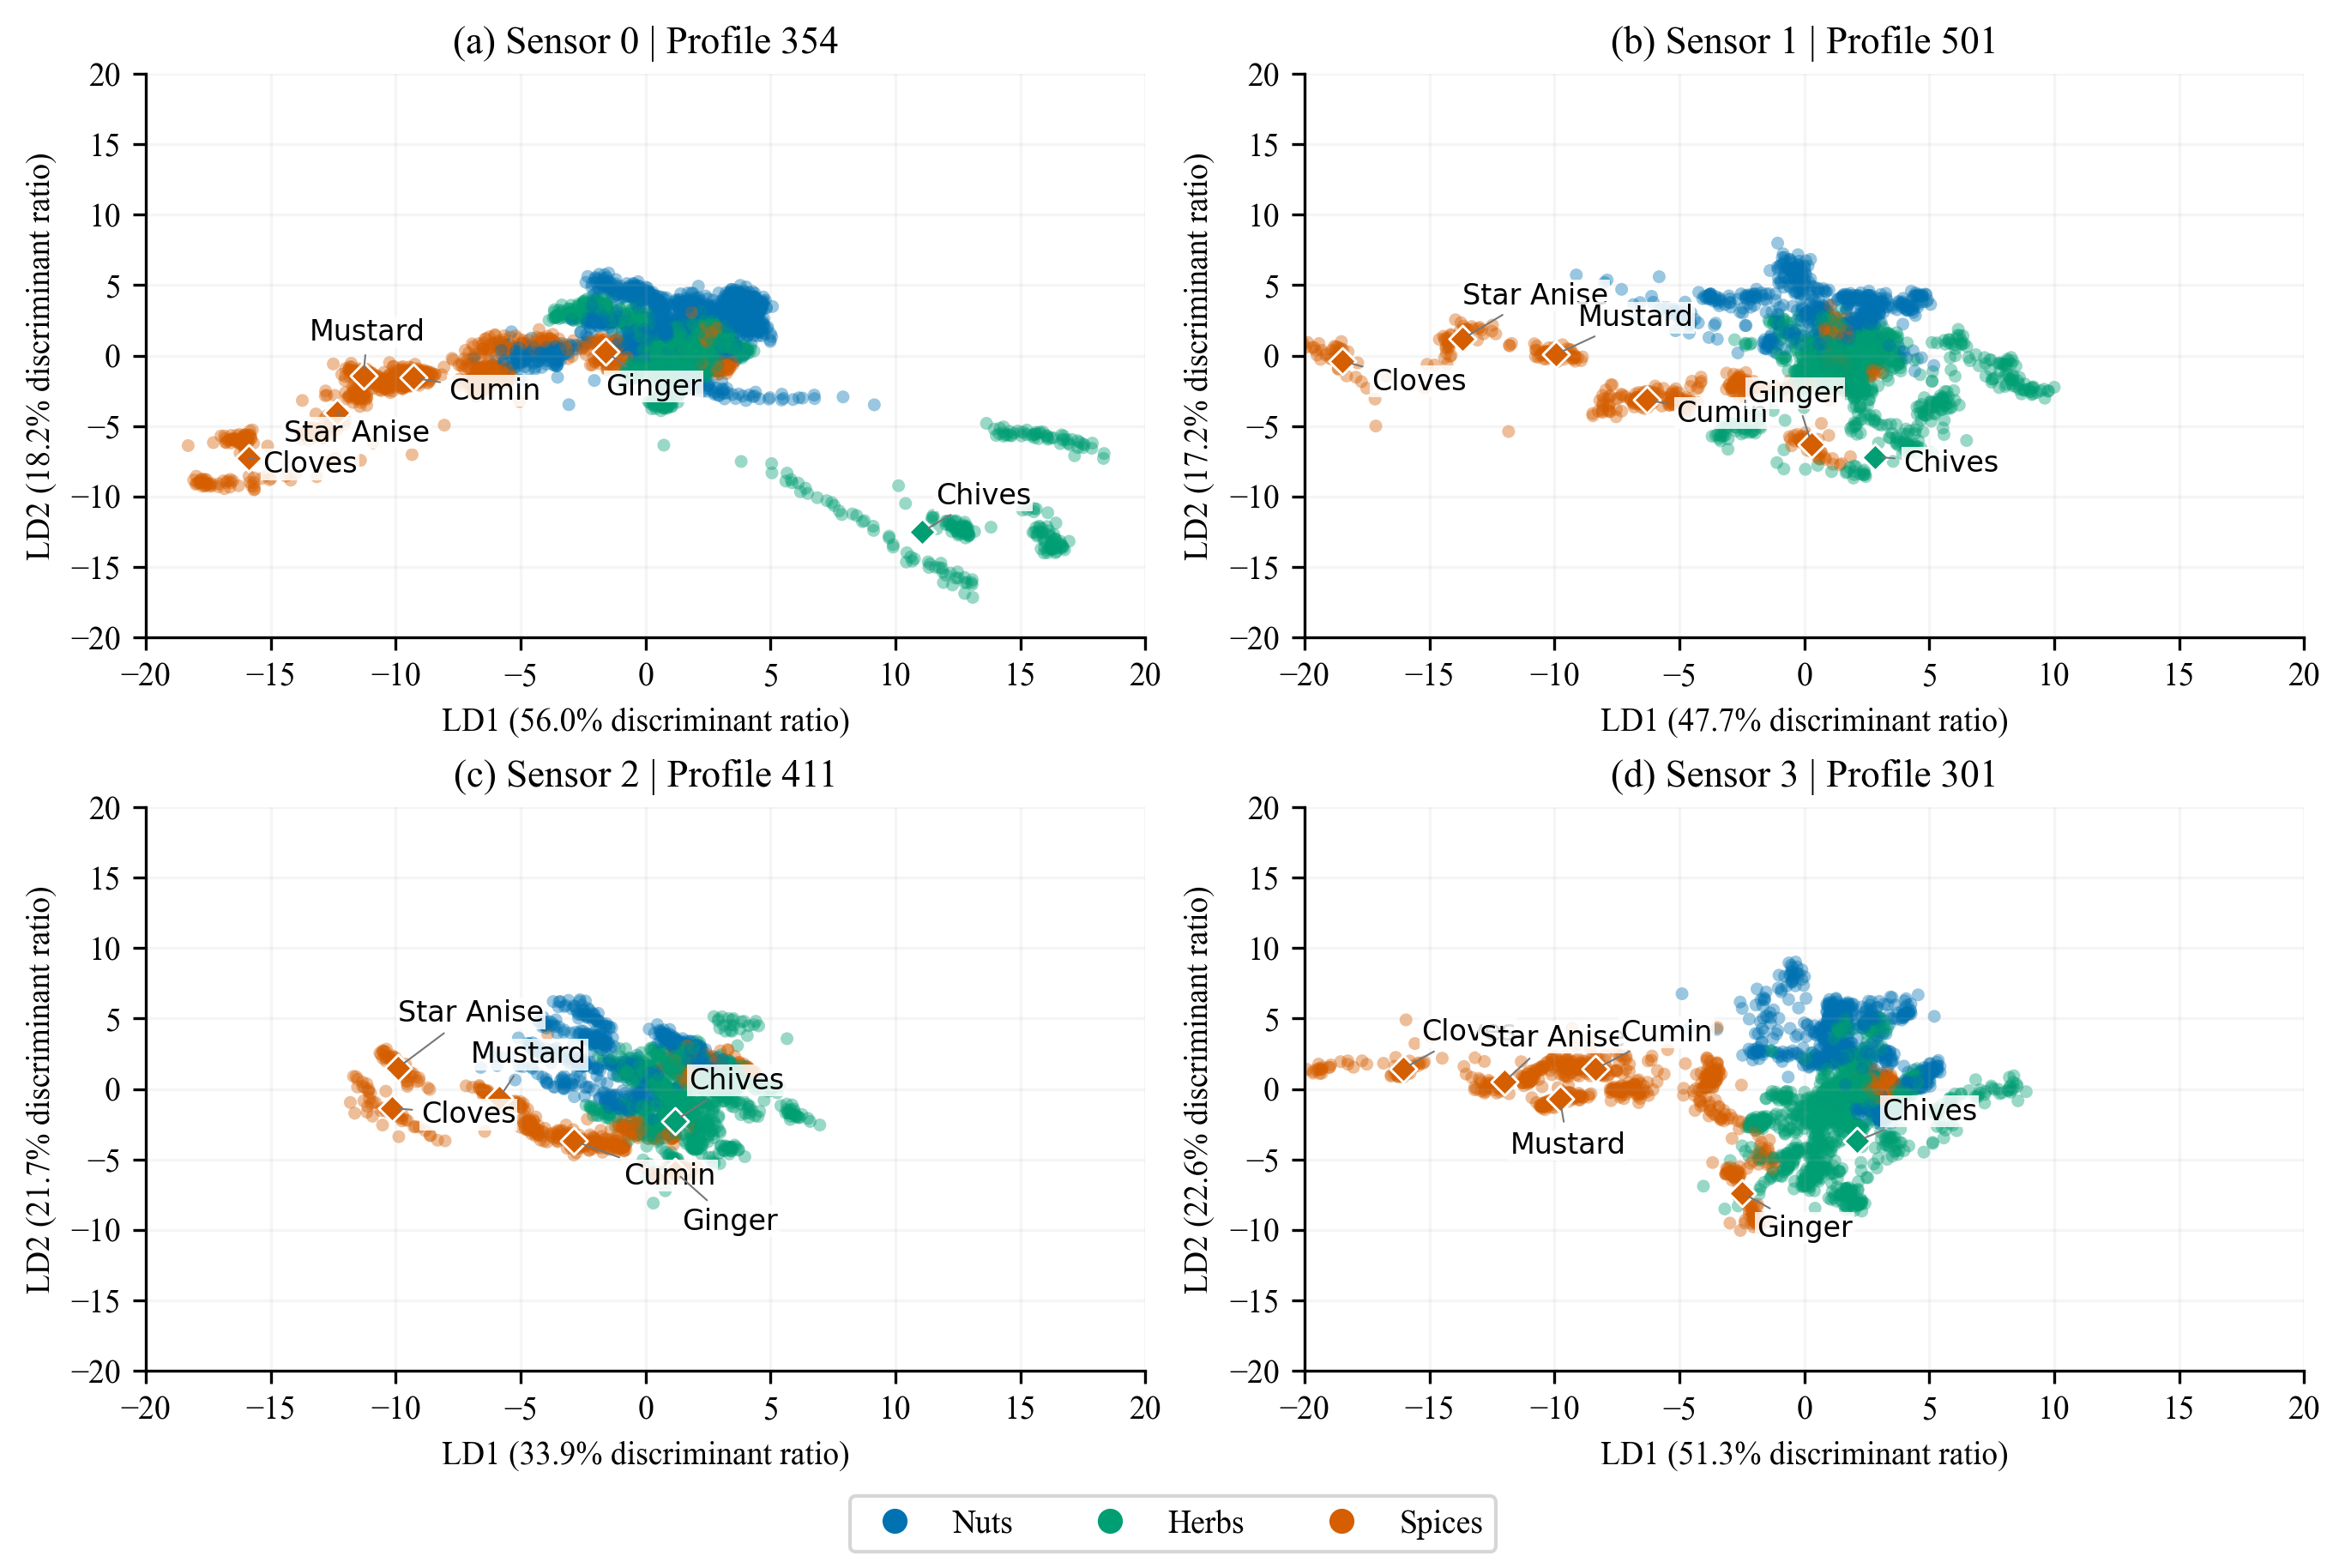
\includegraphics[width=\textwidth]{figures/sensor_pairs_lda.png}
    \caption{Supervised LDA projections for four sensors with different heating profiles. Projections are fitted independently using log-resistance features and substance labels. Points represent measurement cycles, colored by category; labels mark select substance centroids.}
    \label{fig:lda_heating_profiles}
\end{figure*}

Despite being trained on substance labels and not category labels, the projections show partial grouping by category that holds across the different sensors and heating profiles. The aromatic spices form several groups extending away from the main concentration of measurements, while nuts and herbs overlap substantially along LD1 with more variation along LD2. This clustering of the samples by substance category is encouraging, as it suggests alignment between subjective smells and the temperature-cycled MOX sensor signatures.

Fig.~\ref{fig:fingerprints} visualizes the resistance signatures of cumin and lavender for sensors 1 and 5, both using heating profile 501, with different domain adaptation methods. The uncompensated plot in Fig.~\ref{fig:fingerprints}(a) shows clear baseline differences between the sensors, resulting in minimal overlap between the signature distributions for both substances. With CORAL-style adaptation in Fig.~\ref{fig:fingerprints}(b), the signatures of the orange target sensor are brought down to align with the blue source sensor. With vector mean compensation in Fig.~\ref{fig:fingerprints}(c), the signatures for both sensors are transformed by removing the per-step common baseline to create a residual signature. In addition to aligning the distributions, this residual form makes the differences between the cumin and lavender signatures more readily apparent.
\begin{figure*}
    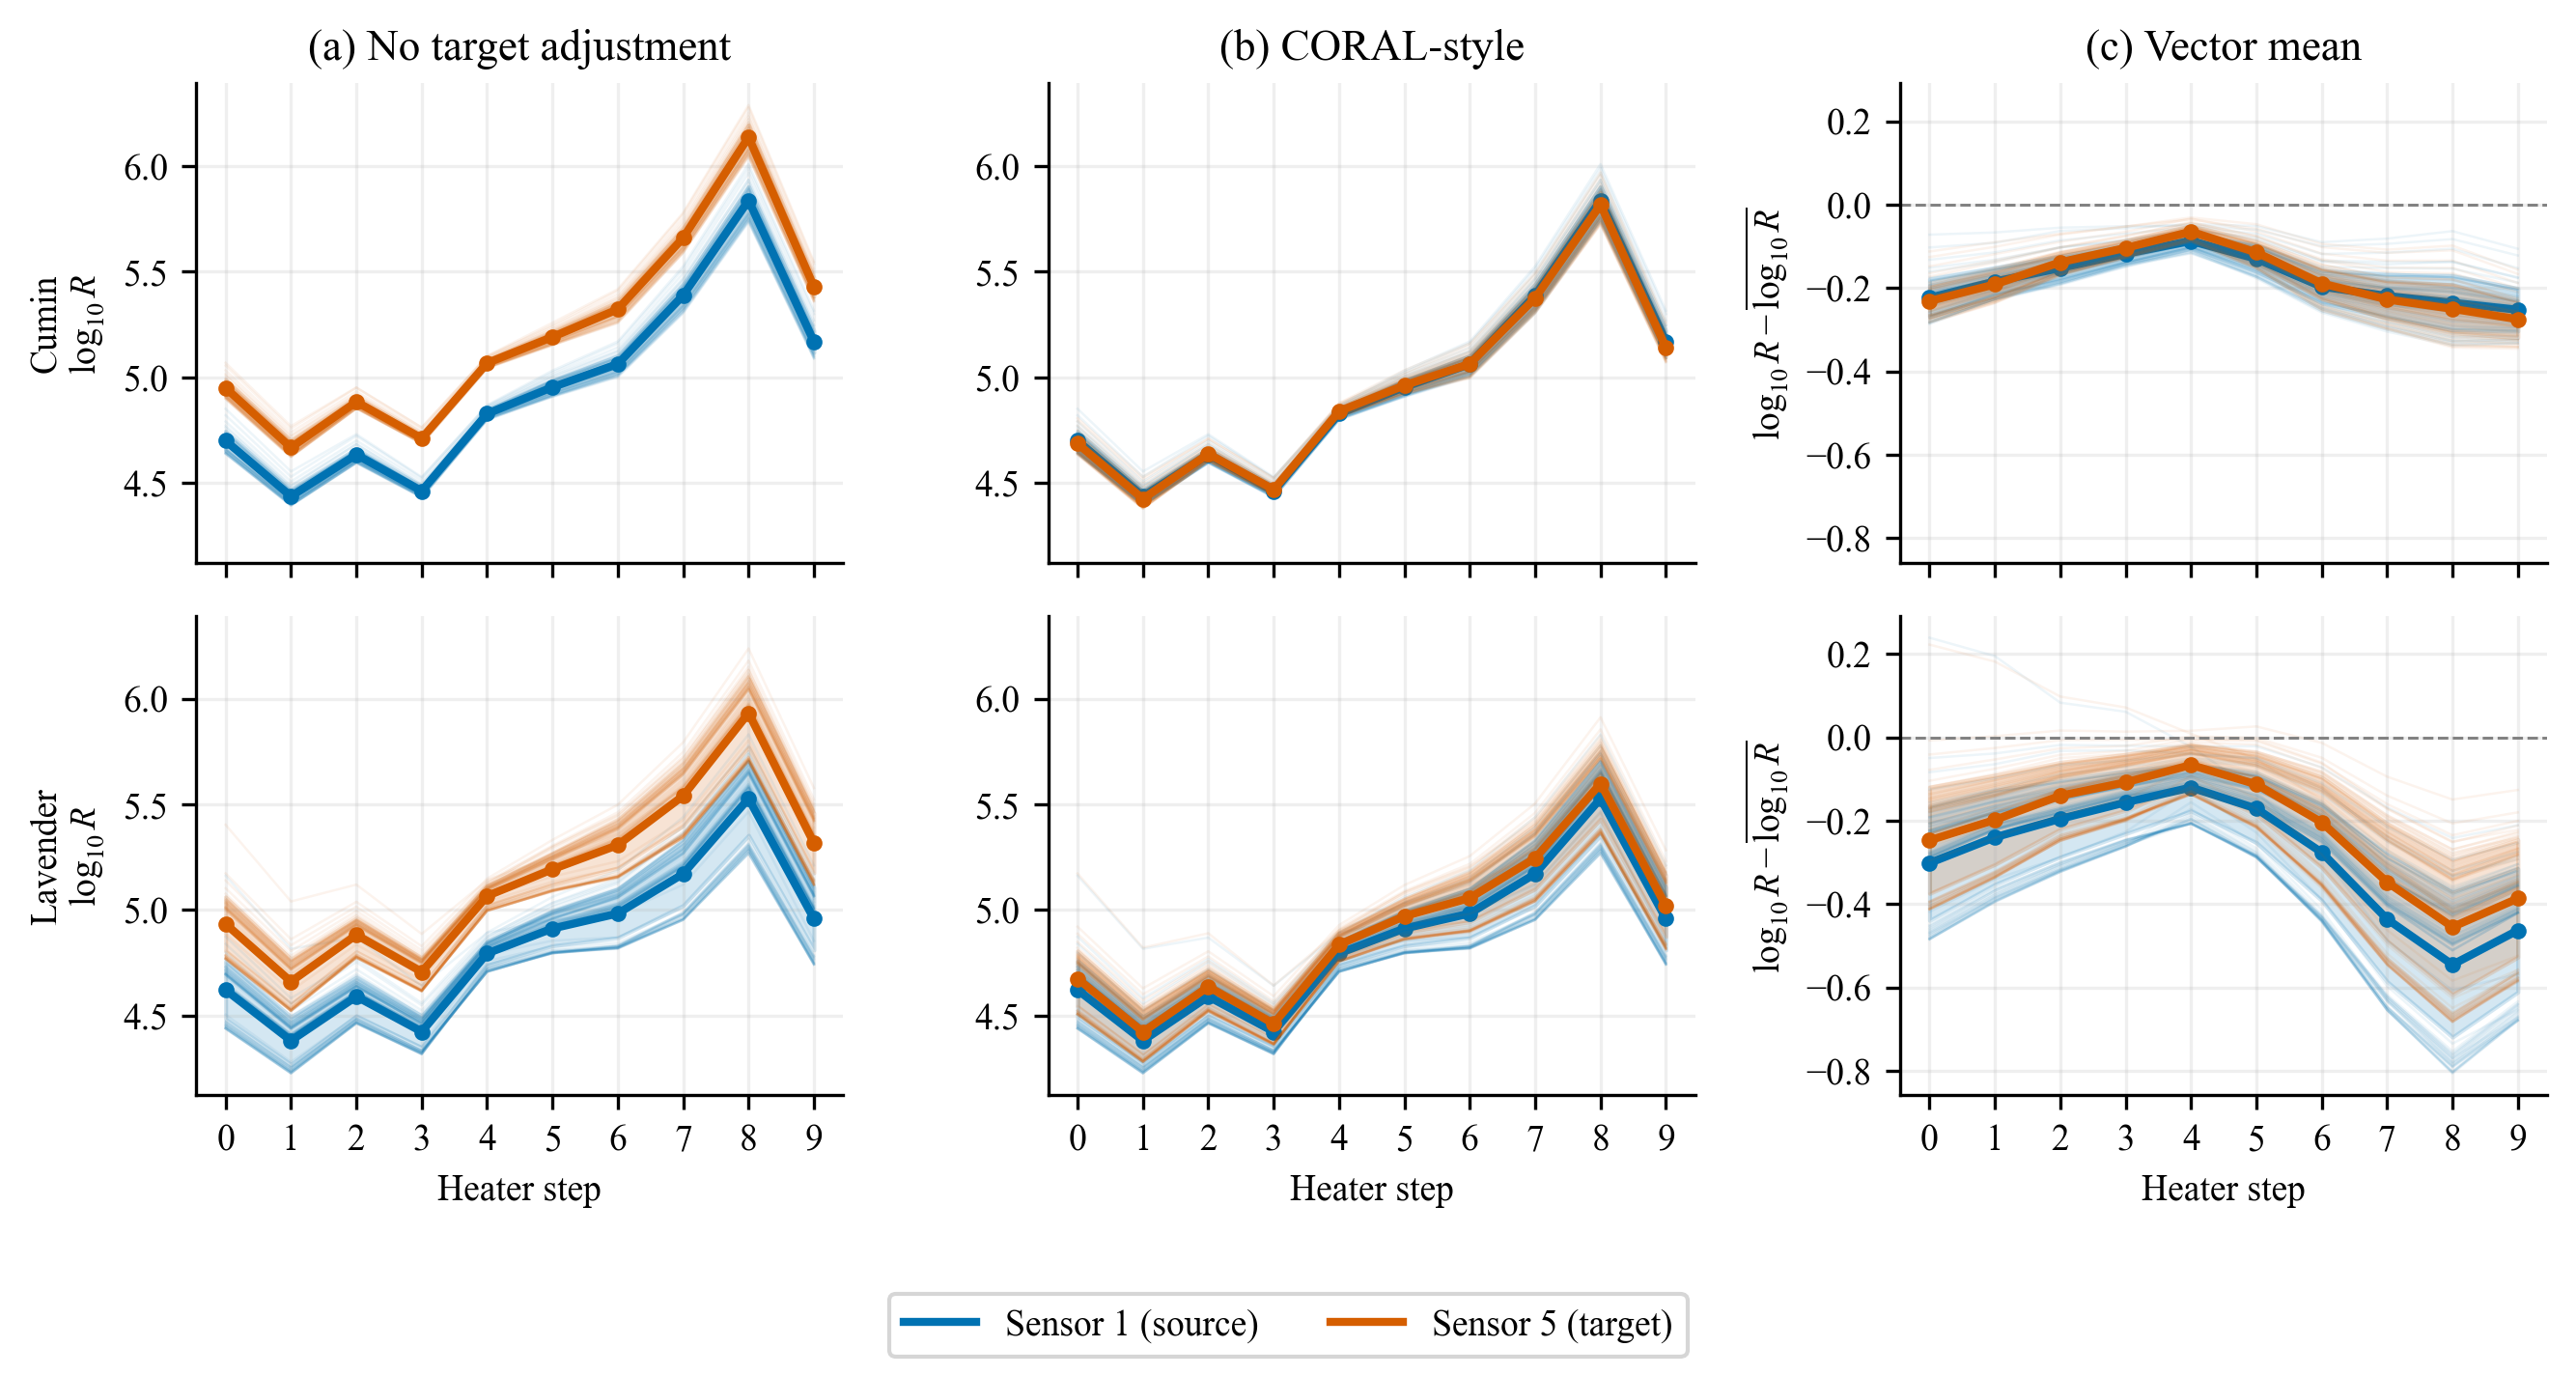
\includegraphics[width=\textwidth]{figures/fingerprints.png}
    \caption{Resistance signatures of cumin (top) and lavender (bottom) for two sensors (1 and 5) with the same heating profile (profile 501) with (a) no domain adaptation, (b) CORAL-style adaptation, and (c) vector mean compensation. Faint lines are individual feature vectors; bold lines are class means.}
    \label{fig:fingerprints}
\end{figure*}

\subsection{Classification Transfer Performance}\label{sec:ablation}
Table \ref{tab:features} summarizes the results of the ablation experiment. The results show that CORAL-style alignment offers the best transfer performance for both feature sets, but per-step compensation accounts for most of the improvement compared to the uncompensated reference.

With log resistance alone, vector mean compensation increases balanced accuracy from 33.8\% to 57.7\%, compared with 37.6\% for scalar mean compensation. Aligning per-feature variances and then the full covariance using CORAL-style adaptation provides smaller additional gains, reaching 59.3\% and 61.7\%, respectively. These methods also reduce variability across transfer directions.

Adding log vapor pressure improves balanced accuracy under every compensation method. CORAL achieves the highest mean balanced accuracy at 71.2\%, exceeding vector mean compensation by 2.8\%, compared with 4.0\% without vapor pressure.

\begin{table}[h]
\centering
\footnotesize
\setlength{\tabcolsep}{3pt}
\caption{Transfer accuracy of LDA classifier with ablation on compensation method and feature inclusion. Scores are reported as mean (SD)\% across all transfer directions. Source accuracy and balanced accuracy on training data are 75.7 (2.6)\% and 80.3 (1.8)\% with log resistance alone; 81.8 (3.1)\% and 85.9 (2.4)\% with vapor pressure included.}
\label{tab:features}
\begin{tabular}{|l|c|c|r|r|}
\hline
 & \multicolumn{2}{|c|}{\textbf{Features}} & \multicolumn{2}{|c|}{\textbf{Target performance}} \\ \cline{2-3}\cline{4-5}
\textbf{Compensation} & \shortstack{\textbf{\textit{Log}}\\\textbf{\textit{resistance}}} & \shortstack{\textbf{\textit{Log vapor}}\\\textbf{\textit{pressure}}} & \textbf{\textit{Accuracy}} & \shortstack{\textbf{\textit{Balanced}}\\\textbf{\textit{accuracy}}} \\
\hline
None & $\times$ & $\checkmark$ & 14.2 (1.4) & 13.6 (1.6) \\
None & $\checkmark$ & $\times$ & 30.6 (9.4) & 33.8 (9.8) \\
None & $\checkmark$ & $\checkmark$ & 42.6 (10.0) & 47.0 (10.0) \\
\hline
Scalar mean & $\checkmark$ & $\times$ & 34.6 (10.7) & 37.6 (10.9) \\
Scalar mean & $\checkmark$ & $\checkmark$ & 45.7 (12.8) & 50.0 (12.9) \\
\hline
Vector mean & $\checkmark$ & $\times$ & 54.3 (4.5) & 57.7 (4.0) \\
Vector mean & $\checkmark$ & $\checkmark$ & 64.5 (4.7) & 68.4 (4.0) \\
\hline
Vector mean-variance & $\checkmark$ & $\times$ & 55.6 (4.5) & 59.3 (4.0) \\
Vector mean-variance & $\checkmark$ & $\checkmark$ & 65.7 (4.9) & 69.8 (3.9) \\
\hline
CORAL-style & $\checkmark$ & $\times$ & 58.0 (3.5) & 61.7 (2.9) \\
CORAL-style & $\checkmark$ & $\checkmark$ & \textbf{67.0 (3.8)} & \textbf{71.2 (3.0)} \\
\hline
\end{tabular}
\end{table}

\subsection{Substance effects}\label{sec:substance}
While Table \ref{tab:features} reports the average accuracy over all substances, the individual results show considerable performance variation between classes. To illustrate this, Table \ref{tab:selected-class-recall} reports the mean, standard deviation, and range across eight transfer directions for selected substances using CORAL-style adaptation with log resistance and vapor pressure features. Mustard, star anise, and dried ginger achieve the highest classification accuracy, with mean recall exceeding 90\% for all sensor pairs, while eupatorium has a mean recall of only 7\%. These class-specific results are consistent with the structure visible in the supervised projections in Fig.~\ref{fig:lda_heating_profiles}, where the aromatic spices mustard, star anise, and ginger are well isolated in several projections, while the herb classes lie close together. This structure is also reflected in the class confusions: eupatorium is most frequently classified as gentiana, while vervain is most frequently classified as rosemary. Similarly, the large range in performance for peanuts and almonds is largely due to confusions between these two classes for sensors 1 and 5. Almond recall is 100\% for the transfer from sensor 1 to sensor 5, but only 4.3\% in the reverse direction, where 42 of 47 almond cycles are classified as peanuts. Conversely, for the sensor 1 to sensor 5 transfer, 23 of 47 peanut samples are misclassified as almond.
These results highlight how sensor-specific variation can shift feature distributions relative to class decision boundaries; a global distribution alignment method such as CORAL can improve average performance while individual classes remain poorly aligned.

\begin{table}[htbp]
\centering
\caption{Recall for selected substances using CORAL and LDA
with log resistance and log vapor pressure. Statistics are
computed across eight transfer directions.}
\label{tab:selected-class-recall}
\footnotesize
\begin{tabular}{|l|r|r|}
\hline
\textbf{Substance} & \textbf{Mean (SD) \%} & \textbf{Range \%} \\
\hline
Mustard    & 98.8 (3.3)  & 90.6--100 \\
Star anise & 98.1 (1.9)  & 93.8--100 \\
Ginger     & 97.7 (2.2)  & 93.4--100 \\
Lavender   & 96.2 (4.1)  & 89.4--99.0 \\
Almond     & 85.0 (33.2) & 4.3--100 \\
Peanuts    & 74.8 (22.4) & 47.1--100 \\
Oregano    & 57.0 (37.5) & 6.2--97.4 \\
Lonicera   & 20.7 (12.5) & 4.1--38.2 \\
Vervain    & 17.7 (14.5) & 4.0--44.1 \\
Eupatorium & 7.0 (6.0)   & 0--16.0 \\
\hline
\end{tabular}
\end{table}

\subsection{Reduced Knowledge Adaptation}
Fig.~\ref{fig:exclusion} plots the target balanced accuracy as we vary the number of classes used for domain adaptation. Fig.~\ref{fig:exclusion}(a) plots the accuracy for all 37 classes, while Fig.~\ref{fig:exclusion}(b) focuses only on those classes that were excluded from the adaptation statistics. Performance for all adaptation methods quickly saturates as the number of classes increases, and the performance on the omitted classes matches the performance across all classes. This is consistent with the results from Section~\ref{sec:ablation},
indicating that the most significant sensor mismatch is a per-heater-step offset in log resistance. The similarity between the all-class results in Fig.~\ref{fig:exclusion}(a) and the excluded class results in Fig.~\ref{fig:exclusion}(b) indicate that the inter-sensor relationship learned from a limited set of substances generalizes across substances to support classification performance. Note that the widening distribution in Fig.~\ref{fig:exclusion}(b) does not necessarily indicate less stable adaptation: as adaptation coverage increases, fewer classes remain omitted, making their average recall more sensitive to the per-class differences described in Section~\ref{sec:substance}.

\begin{figure}[tpb]
    \centering
    %\includegraphics[width=\linewidth]{../results/substance_exclusion/coverage.png}
    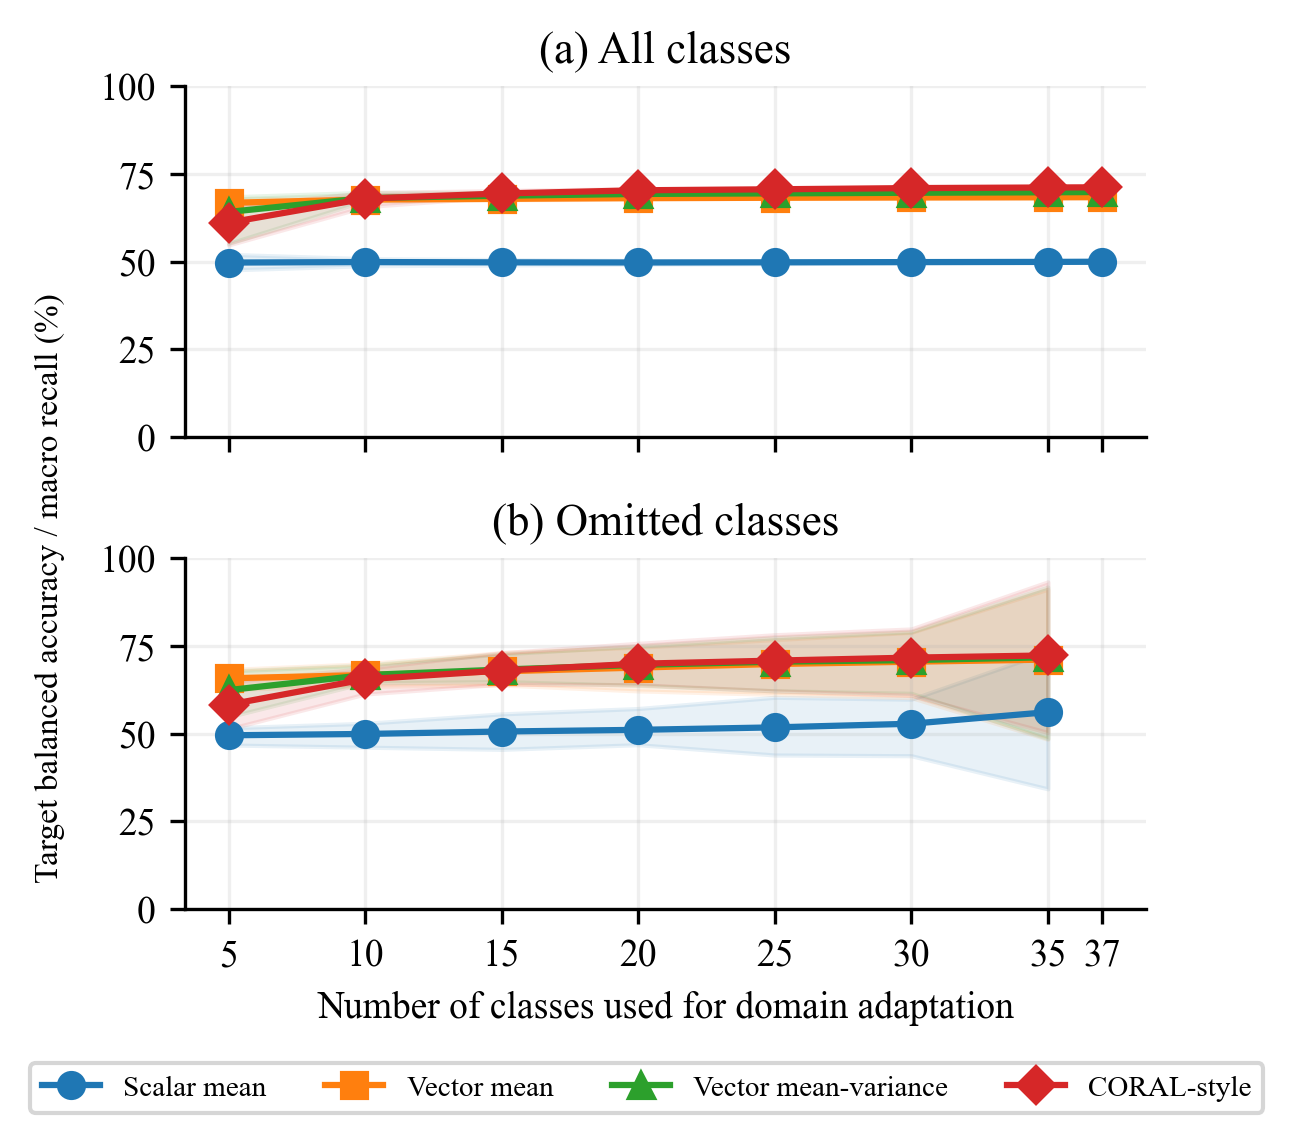
\includegraphics[width=\linewidth]{figures/domain_adaptation.png}
    \caption{Target performance using resistance and vapor pressure features, varying the number of classes for domain adaptation. Balanced accuracy for (a) all classes, and (b) classes excluded from adaptation. Lines show the averages and bands show the 10th–90th percentiles across 30 trials.}
    \label{fig:exclusion}
\end{figure}

\section{Conclusion}
This study demonstrates improved classification transfer between temperature-modulated MOX sensors using compensation estimated from unlabeled exposure data. Per-heater-step mean compensation provides much of the improvement over uncompensated transfer, with variance and covariance alignment yielding additional gains. Including vapor pressure improves performance under every evaluated compensation method.

Per-step mean compensation retains most of its full-coverage performance when adaptation statistics are estimated from only five substances. This motivates future work on estimating and updating the per-step means online from unlabeled measurements to account for sensor drift.

A limitation of this study is that source and target sensors were measured simultaneously under shared exposure conditions. Further evaluation is needed under different exposure histories and environmental conditions, where online estimation must distinguish sensor drift from changes in the exposure mixture.

\section*{Acknowledgment}
This work was supported by the National Research Council Canada (NRC) New Beginnings Initiative.

\printbibliography

\end{document}
